\sloppy
\section{Results}\label{sec:results}

All test numbers are nDCG on uniformly exposed test data. Validation and test splits are drawn from the
uniform data; the training log is the only data used to fit the nuisances and the model. For each
dataset and split, the final method (\qp) is the validated combination of its jobs: each split keeps the
job, offset weight and epoch with the best validation score. Table~\ref{tab:main} reports the main run
(seed 0), Table~\ref{tab:seeds} the retraining with seeds 1--3, and the remaining tables the ablations
and the walk-correction analysis. Per-user paired tests use the users who appear in the test sets of
both methods: 225 on Coat, 2{,}310 on Yahoo! R3, 8{,}321 on KuaiRand and 1{,}410 on KuaiRec.

\subsection{Main comparison}\label{sec:main}

Table~\ref{tab:main} and Figure~\ref{fig:forest} give the main comparison.

\begin{enumerate}
\item \textbf{Graph baselines.} On all four datasets the final method has a higher mean than every graph
baseline we ran: LightGCN, r-AdjNorm~\citep{zhao2022radjnorm}, NAVIP~\citep{kim2022navip}, SimGCL~\citep{yu2022simgcl}
and the AdvInfoNCE re-implementation. DR-LightGCN is in the Holm family only on Coat and KuaiRec; on
Yahoo! R3 and KuaiRand it was not tested for the final method. Every paired difference against a graph baseline is
significant ($p_{\text{Holm}}\le0.0185$) except one: LightGCN-pt on KuaiRec, $+1.31$ [3.34], $p_{\text{Holm}}=0.4409$.
Apart from LightGCN-pt, the largest adjusted p-value is $0.0185$ (KuaiRand, r-AdjNorm).
\item \textbf{Yahoo! R3.} The final method reaches $0.6866$ against $0.6742$ for r-AdjNorm, the strongest
baseline, a paired difference of $+12.67$ [6.01] ($\times10^{-3}$, $p_{\text{Holm}}<0.001$). It is the best
method we ran on this dataset. The training-free DR adjacency and DRUP rows (0.6567) and the DR-JL and MRDR
rows (about 0.52) are below it; these rows were not tested in the Holm family.
\item \textbf{KuaiRand.} The final method reaches $0.4613$ against $0.4590$ for r-AdjNorm, a paired difference of
$+1.94$ [1.61] ($p_{\text{Holm}}=0.0185$). The effect is small. Validation chose $\beta=0$ in four of five splits,
so in the selected runs the gain comes mainly from the weighting. The $\beta=0$ job alone reaches $0.4623$ on the test set, above
the validated combination, so the validation choice is not always the test-best choice.
\item \textbf{Coat.} The final method reaches $0.6015$ against $0.5812$ for iALS, $+20.02$ [19.74]
($p_{\text{Holm}}=0.0469$) in the main run. This difference does not survive retraining (Section~\ref{sec:seeds}),
and the difference from iALS is not significant across seeds.
\item \textbf{KuaiRec.} The final method reaches $0.6285$. It is below DR-JL ($0.6332$; $-4.56$ [2.24],
$p_{\text{Holm}}<0.001$) and MRDR ($0.6328$; $-4.34$ [2.16], $p_{\text{Holm}}<0.001$), and below the training-free
DR adjacency and DRUP operators ($0.6378$, not tested). Apart from DR-JL and MRDR it has the highest mean in
the family, but the difference to LightGCN-pt is not significant. Section~\ref{sec:walk} discusses the training-free
operators.
\item \textbf{Scale.} Against the strongest graph baseline by mean, the paired differences are $+32.68$ (Coat,
DR-LightGCN), $+12.67$ (Yahoo! R3, r-AdjNorm), $+1.94$ (KuaiRand, r-AdjNorm) and $+1.31$ (KuaiRec,
LightGCN-pt, not significant), in units of $10^{-3}$ nDCG. The paired differences therefore range from
$1.3$ to $32.7$ thousandths of nDCG.
\end{enumerate}

\begin{figure}[t]
\centering
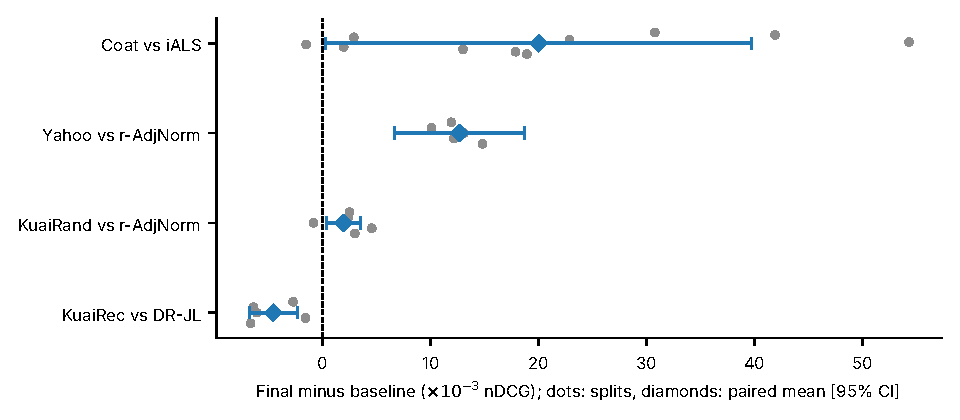
\includegraphics[width=\linewidth]{figs/fig_forest}
\caption{Per-split test difference between the final method and the strongest baseline of each dataset
(Coat: iALS; Yahoo! R3 and KuaiRand: r-AdjNorm; KuaiRec: DR-JL). Dots are the splits (five, or ten on
Coat); diamonds are the paired per-user mean difference from Table~\ref{tab:main} with its 95\% CI
half-width. Units are $\times10^{-3}$ nDCG.}
\label{fig:forest}
\end{figure}

% Table 2: main comparison. Sources: results/v4/final_summary.txt (method and paired diffs, p_Holm,
% configuration counts), paper/tables/accuracy.tex (sd of baselines and extra rows), ensemble_summary
% and final_analysis (sd of the final method). Diff = paired per-user mean difference (final minus
% baseline) x 1e-3, 95% CI half-width in brackets.
\begin{table}[t]
\centering
\caption{Main comparison (seed 0, full selection). Test nDCG is mean $\pm$ sd over splits. Diff is the paired per-user difference of the final method minus the baseline, $\times10^{-3}$, with the 95\% CI half-width. $p_{\text{Holm}}$ is adjusted within each dataset over the block's family (sizes 8, 6, 7, 9). Bold: best of the block; underline: second (KuaiRec: within the family). The final method is tuned over 324, 84, 30 and 120 configurations (Coat, Yahoo! R3, KuaiRand, KuaiRec), against 6 to 216 for the baselines (Configs column). Rows marked re-impl.\ use a simplified AdvInfoNCE (Section~\ref{sec:advsetup}). On KuaiRec the final method ranks third within its Holm family.}
\label{tab:main}
\footnotesize
\setlength{\tabcolsep}{4pt}
\renewcommand{\arraystretch}{0.9}
\begin{tabular}{@{}lrrrr@{}}
\toprule
Method & Test nDCG & Configs & Diff $\times10^{-3}$ [95\% CI] & $p_{\text{Holm}}$ \\
\midrule
\multicolumn{5}{@{}l}{\emph{Coat (nDCG@5; 10 splits)}} \\
\qp (final) & \textbf{0.6015 $\pm$ 0.0162} & 324 & -- & -- \\
iALS & \underline{0.5812 $\pm$ 0.0101} & 24 & $+20.02$ [19.74] & 0.0469 \\
DR-LightGCN & 0.5724 $\pm$ 0.0205 & 54 & $+32.68$ [23.12] & 0.0116 \\
r-AdjNorm & 0.5722 $\pm$ 0.0134 & 108 & $+28.27$ [18.42] & 0.0083 \\
LightGCN & 0.5683 $\pm$ 0.0132 & 54 & $+32.03$ [17.27] & 0.0016 \\
NAVIP & 0.5664 $\pm$ 0.0163 & 54 & $+33.62$ [19.63] & 0.0035 \\
SimGCL & 0.5528 $\pm$ 0.0141 & 108 & $+49.52$ [23.99] & 0.0004 \\
MACR & 0.5418 $\pm$ 0.0134 & 36 & $+61.46$ [27.66] & $<0.001$ \\
AdvInfoNCE (re-impl.) & 0.5222 $\pm$ 0.0204 & 216 & $+78.50$ [27.63] & $<0.001$ \\
\midrule
\multicolumn{5}{@{}l}{\emph{Yahoo! R3 (nDCG@5; 5 splits)}} \\
\qp (final) & \textbf{0.6866 $\pm$ 0.0034} & 84 & -- & -- \\
r-AdjNorm & \underline{0.6742 $\pm$ 0.0047} & 72 & $+12.67$ [6.01] & $<0.001$ \\
LightGCN & 0.6708 $\pm$ 0.0061 & 36 & $+16.77$ [5.82] & $<0.001$ \\
NAVIP & 0.6701 $\pm$ 0.0039 & 36 & $+17.51$ [6.02] & $<0.001$ \\
iALS & 0.6625 $\pm$ 0.0043 & 12 & $+24.88$ [8.77] & $<0.001$ \\
AdvInfoNCE (re-impl.) & 0.6477 $\pm$ 0.0048 & 16 & $+37.85$ [8.48] & $<0.001$ \\
SimGCL & 0.6348 $\pm$ 0.0048 & 12 & $+53.26$ [10.05] & $<0.001$ \\
\midrule
\multicolumn{5}{@{}l}{\emph{KuaiRand (nDCG@10; 5 splits)}} \\
\qp (final) & \textbf{0.4613 $\pm$ 0.0024} & 30 & -- & -- \\
r-AdjNorm & \underline{0.4590 $\pm$ 0.0024} & 12 & $+1.94$ [1.61] & 0.0185 \\
LightGCN & 0.4569 $\pm$ 0.0010 & 6 & $+3.93$ [1.53] & $<0.001$ \\
NAVIP & 0.4565 $\pm$ 0.0017 & 6 & $+4.36$ [1.46] & $<0.001$ \\
iALS & 0.4528 $\pm$ 0.0017 & 12 & $+8.98$ [3.23] & $<0.001$ \\
AdvInfoNCE (re-impl.) & 0.4480 $\pm$ 0.0017 & 8 & $+12.79$ [2.50] & $<0.001$ \\
BPR-MF & 0.4475 $\pm$ 0.0027 & 6 & $+13.99$ [2.62] & $<0.001$ \\
SimGCL & 0.4196 $\pm$ 0.0022 & 12 & $+42.20$ [4.04] & $<0.001$ \\
\midrule
\multicolumn{5}{@{}l}{\emph{KuaiRec (nDCG@20; 5 splits)}} \\
\textbf{DR-JL} & \textbf{0.6332 $\pm$ 0.0026} & 6 & $-4.56$ [2.24] & $<0.001$ \\
MRDR & \underline{0.6328 $\pm$ 0.0020} & 6 & $-4.34$ [2.16] & $<0.001$ \\
\qp (final) & 0.6285 $\pm$ 0.0022 & 120 & -- & -- \\
LightGCN-pt & 0.6271 $\pm$ 0.0023 & 36 & $+1.31$ [3.34] & 0.4409 \\
DR-LightGCN & 0.6212 $\pm$ 0.0071 & 6 & $+7.73$ [2.01] & $<0.001$ \\
NAVIP & 0.6186 $\pm$ 0.0024 & 6 & $+10.49$ [2.28] & $<0.001$ \\
iALS & 0.6133 $\pm$ 0.0027 & 12 & $+15.92$ [3.03] & $<0.001$ \\
LightGCN & 0.6085 $\pm$ 0.0028 & 36 & $+20.90$ [2.88] & $<0.001$ \\
r-AdjNorm & 0.6083 $\pm$ 0.0031 & 12 & $+20.68$ [2.75] & $<0.001$ \\
AdvInfoNCE (re-impl.) & 0.5776 $\pm$ 0.0036 & 8 & $+49.32$ [6.57] & $<0.001$ \\
\bottomrule
\end{tabular}
\\[2pt]
{\footnotesize Beta per split: Coat 1.0 (5 splits), 2.0 (2), 0.5 (1), 0.0 (2); Yahoo! R3 1.0 (4), 0.0 (1); KuaiRand 0.0 (4), 0.5 (1); KuaiRec 1.0 (4), 2.0 (1). Training-free and other rows: Table~\ref{tab:extra}.}
\end{table}


% Table 2b: rows of Table 2 outside the Holm families (not tested against the final method). Means and sd
% (ddof $=0$) from paper/tables/accuracy.tex of the same runs.
\begin{table}[t]
\centering
\caption{Training-free and other methods outside the Holm families of Table~\ref{tab:main}. Their differences
to the final method were not tested. Test nDCG is mean $\pm$ sd over splits. DR adjacency is the doubly robust
operator without the walk correction; DRUP adds the walk correction. On Yahoo! R3 and KuaiRand, DRUP, DR adjacency and
IPS adjacency have identical means.}
\label{tab:extra}
\small
\begin{tabular}{@{}llr@{}}
\toprule
Dataset & Method & Test nDCG \\
\midrule
Coat (nDCG@5) & DRUP & 0.5467 $\pm$ 0.0235 \\
 & DR adjacency & 0.5459 $\pm$ 0.0244 \\
 & MRDR & 0.4869 $\pm$ 0.0187 \\
 & DR-JL & 0.4811 $\pm$ 0.0164 \\
\midrule
Yahoo! R3 (nDCG@5) & DRUP & 0.6567 $\pm$ 0.0063 \\
 & DR adjacency & 0.6567 $\pm$ 0.0063 \\
 & DR-LightGCN & 0.5528 $\pm$ 0.0091 \\
 & MRDR & 0.5248 $\pm$ 0.0059 \\
 & DR-JL & 0.5225 $\pm$ 0.0043 \\
\midrule
KuaiRand (nDCG@10) & DRUP & 0.4492 $\pm$ 0.0013 \\
 & DR adjacency & 0.4492 $\pm$ 0.0013 \\
 & DR-JL & 0.3759 $\pm$ 0.0021 \\
\midrule
KuaiRec (nDCG@20) & DRUP & \textbf{0.6378 $\pm$ 0.0019} \\
 & DR adjacency & \underline{0.6378 $\pm$ 0.0020} \\
\bottomrule
\end{tabular}
\end{table}


\subsection{Robustness to the training seed}\label{sec:seeds}

Table~\ref{tab:seeds} retrains the selected configuration of every split with seeds 1, 2 and 3 and
re-selects only the epoch on validation data. Seed 0 is the main run. Each dataset has a Holm family of two
comparisons against its two strongest baselines in the main run, chosen by main-run test mean (Section~\ref{sec:seedsetup}).

On Coat the seed-averaged final method reaches $0.5911\pm0.0049$ against $0.5862\pm0.0029$ for iALS. The paired
difference is $+3.39$ [20.70] with $p_{\text{Holm}}=0.747$, which is not significant. The Coat claim is therefore
that the difference from iALS is not significant across seeds. Against DR-LightGCN the difference remains large and significant
($+33.36$ [17.31], $p_{\text{Holm}}=0.0004$). The spread of the final method across seeds on Coat (sd 0.0049,
ddof $=0$) is larger than that of iALS (0.0029), and the seed-0 value of $0.6015$ is the highest of the four
seeds. The main-run advantage over iALS on Coat should therefore be read as a single-run result.

On Yahoo! R3 the seed-averaged final method reaches $0.6881\pm0.0005$, against $0.6736$ for r-AdjNorm
($+14.76$ [5.23], $p_{\text{Holm}}<0.001$) and $0.6691$ for LightGCN ($+20.02$ [5.08], $p_{\text{Holm}}<0.001$).
On KuaiRand it reaches $0.4604\pm0.0003$, against $0.4580$ for r-AdjNorm ($+2.31$ [1.23], $p_{\text{Holm}}=0.0002$)
and $0.4555$ for LightGCN ($+4.87$ [1.12], $p_{\text{Holm}}<0.001$). Both gains are small in absolute terms.

On KuaiRec the seed-averaged final method reaches $0.6290\pm0.0002$, against $0.6298$ for DR-JL and $0.6304$
for MRDR. The differences are $-1.03$ [1.64] ($p_{\text{Holm}}=0.2213$) and $-1.56$ [1.47] ($p_{\text{Holm}}=0.0760$).
The significant deficit of the main run therefore becomes a gap of $1.0$ to $1.6$ thousandths of nDCG that is not
significant over the retraining seeds, although the seed-averaged mean is lower than both. Both statements are reported: below DR-JL and MRDR in the main run, and not
significantly different from them across retraining seeds.

% Table 4: seed robustness. Source: results/v4/seeds_summary.txt (lines 3-41). The seed-0 column is the
% main run of Table 2. Mean and sd are over seeds 1-3 (ddof $=0$); the last column is the sample sd (ddof $=1$).
\begin{table}[t]
\centering
\caption{Robustness to the training seed. Seed 0 is the main run of Table~\ref{tab:main}; seeds 1--3 retrain
the selected configuration of each split and re-select only the epoch on validation data. Test nDCG
per seed is the mean over splits. Each dataset has a Holm family of two paired comparisons (the two
strongest baselines of the main run). The two baselines of each dataset are the two highest-scoring baselines of the main run by test mean, and they are retrained with seeds 1--3 in the same way as the final method. Diff is the paired per-user mean difference (not the difference of the two table means), $\times10^{-3}$, with the 95\% CI half-width in brackets.}
\label{tab:seeds}
\footnotesize
\setlength{\tabcolsep}{2.5pt}
\begin{tabular}{@{}lrrrrrr@{}}
\toprule
Method & Seed 0 & Seed 1 & Seed 2 & Seed 3 & Mean $\pm$ sd (1--3) & sd (ddof 1) \\
\midrule
\multicolumn{7}{@{}l}{\emph{Coat (nDCG@5)}} \\
\qp (final) & 0.6015 & 0.5980 & 0.5879 & 0.5874 & 0.5911 $\pm$ 0.0049 & 0.0060 \\
iALS & 0.5812 & 0.5900 & 0.5829 & 0.5858 & 0.5862 $\pm$ 0.0029 & 0.0036 \\
DR-LightGCN & 0.5724 & 0.5550 & 0.5632 & 0.5645 & 0.5609 $\pm$ 0.0042 & 0.0051 \\
\multicolumn{7}{@{}l}{\quad vs iALS: $+3.39$ [20.70], $p_{\text{Holm}}=0.747$} \\
\multicolumn{7}{@{}l}{\quad vs DR-LightGCN: $+33.36$ [17.31], $p_{\text{Holm}}=0.0004$} \\
\midrule
\multicolumn{7}{@{}l}{\emph{Yahoo! R3 (nDCG@5)}} \\
\qp (final) & 0.6866 & 0.6874 & 0.6882 & 0.6886 & 0.6881 $\pm$ 0.0005 & 0.0006 \\
r-AdjNorm & 0.6742 & 0.6711 & 0.6752 & 0.6746 & 0.6736 $\pm$ 0.0018 & 0.0022 \\
LightGCN & 0.6708 & 0.6671 & 0.6700 & 0.6702 & 0.6691 $\pm$ 0.0014 & 0.0018 \\
\multicolumn{7}{@{}l}{\quad vs r-AdjNorm: $+14.76$ [5.23], $p_{\text{Holm}}<0.001$} \\
\multicolumn{7}{@{}l}{\quad vs LightGCN: $+20.02$ [5.08], $p_{\text{Holm}}<0.001$} \\
\midrule
\multicolumn{7}{@{}l}{\emph{KuaiRand (nDCG@10)}} \\
\qp (final) & 0.4613 & 0.4602 & 0.4601 & 0.4608 & 0.4604 $\pm$ 0.0003 & 0.0004 \\
r-AdjNorm & 0.4590 & 0.4582 & 0.4576 & 0.4582 & 0.4580 $\pm$ 0.0003 & 0.0003 \\
LightGCN & 0.4569 & 0.4557 & 0.4547 & 0.4561 & 0.4555 $\pm$ 0.0006 & 0.0007 \\
\multicolumn{7}{@{}l}{\quad vs r-AdjNorm: $+2.31$ [1.23], $p_{\text{Holm}}=0.0002$} \\
\multicolumn{7}{@{}l}{\quad vs LightGCN: $+4.87$ [1.12], $p_{\text{Holm}}<0.001$} \\
\midrule
\multicolumn{7}{@{}l}{\emph{KuaiRec (nDCG@20)}} \\
\qp (final) & 0.6285 & 0.6292 & 0.6287 & 0.6291 & 0.6290 $\pm$ 0.0002 & 0.0003 \\
DR-JL & 0.6332 & 0.6304 & 0.6308 & 0.6283 & 0.6298 $\pm$ 0.0011 & 0.0013 \\
MRDR & 0.6328 & 0.6305 & 0.6291 & 0.6315 & 0.6304 $\pm$ 0.0010 & 0.0012 \\
\multicolumn{7}{@{}l}{\quad vs DR-JL: $-1.03$ [1.64], $p_{\text{Holm}}=0.2213$} \\
\multicolumn{7}{@{}l}{\quad vs MRDR: $-1.56$ [1.47], $p_{\text{Holm}}=0.0760$} \\
\bottomrule
\end{tabular}
\end{table}


\subsection{Where does the gain come from?}\label{sec:ablations}

Table~\ref{tab:ablation} and Figure~\ref{fig:ablation} separate the two ingredients: the weights on the
sampled negatives and the fixed offset. Each row is one stored job. The rows are not matched in their
configuration grids, and the ablation rows carry no significance tests. The one test in this section is the KuaiRec decomposition test below.

\paragraph{Weights.} On Coat the full weighting (Q-LightGCN, no offset) reaches $0.5912$, against $0.5683$
for LightGCN. Replacing Q by the imputation alone, $\hat Y$, gives $0.5937$; replacing it by rescaled item
popularity gives $0.5751$; and a random permutation of the Q values, which keeps their marginal distribution,
gives $0.5689$, the LightGCN level. On Yahoo! R3 the weighted model reaches $0.6829$ (learning rate $3\times10^{-3}$
only), against $0.6708$ for LightGCN, popularity-only weights give $0.6550$, and the shuffled control gives
$0.6689$. The shuffled control removes the gain on both datasets, so the gain is not a rescaling effect of the
weights. Popularity-only weights are weaker than Q on both datasets, and on Yahoo! R3 they are below LightGCN.
On Coat, dropping the propensity from Q changes little ($0.5937$ against $0.5912$), so in this comparison the information appears to lie in the
imputation. This is an observation only: the grids are not matched and no test was run. The Coat weighted runs use 108 configurations (with $\mathrm{fn}\in\{0.5,1\}$) against 54 for the
ablations, so these two numbers are not grid-matched.

\paragraph{Offset.} On Coat, LightGCN with the offset only (P-LightGCN, $\beta\in\{0.5,1\}$)
reaches $0.6020$, with the weights as well $0.6039$ ($\beta\in\{0.5,1\}$) and $0.6046$ ($\beta\in\{1,2\}$), and the
validated combination $0.6015$. On Coat, with unmatched grids and no test, the offset alone recovers essentially all of the gain, and the
weighting adds little on top of it ($0.6020$ against $0.6039$). On KuaiRec, with the same grid as the weighted run with the offset
($\beta\in\{0.5,1\}$, one learning rate), the offset alone reaches nDCG@20 $0.6288$ and the weighted run with the offset
$0.6281$, so the weighting adds nothing there either. Offset-only runs for Yahoo! R3 and KuaiRand were not completed and are untested.

\paragraph{Imputation model.} On Coat a rank-16 low-rank imputation for Q and the offset gives $0.5887$ without
offset and $0.5897$ with it, against $0.5912$ and $0.6039$ for the additive imputation. The more flexible model
is worse on this dataset. Q-iALS, iALS with the same weights, reaches $0.5871$ against $0.5812$ for iALS, using
48 and 24 configurations. It was not run on the larger datasets, where the dense solve is too slow. We report
the Q-iALS result as an observation and make no significance claim.

\paragraph{Decomposition across datasets.} Table~\ref{tab:decomp} compares the weighting-only
selection with the validated combination on every dataset. On Yahoo! R3 the weighting-only selection reaches
$0.6837$ and the combination $0.6866$; on KuaiRand $0.4623$ (the $\beta=0$ job) against $0.4613$; on KuaiRec
$0.6095$ against $0.6285$. Read this way, the weighting carries most of the Yahoo! R3 and KuaiRand results.
On KuaiRec the validated combination exceeds the weighting-only selection by $0.019$. This is a decomposition of selected runs rather than a
matched ablation. On KuaiRec the weighting alone is not significantly better than LightGCN ($+1.39$ [1.38],
$p_{\text{Holm}}=0.0967$) and has a lower mean than NAVIP, DR-LightGCN and iALS.

\begin{figure}[t]
\centering
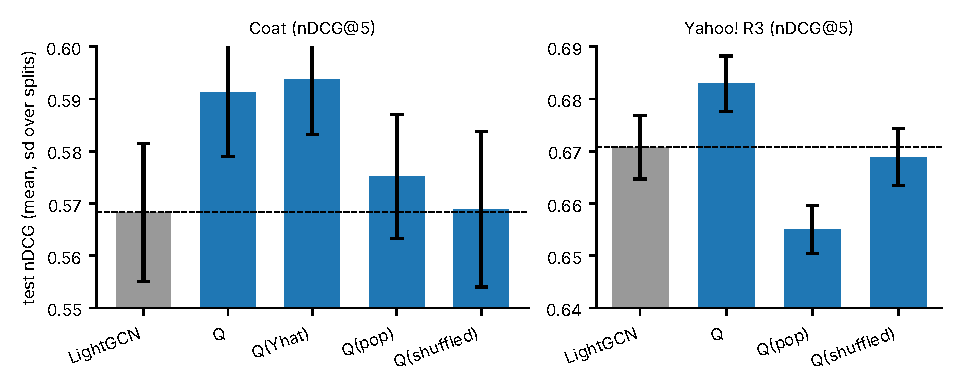
\includegraphics[width=\linewidth]{figs/fig_ablation}
\caption{Ablations of the weights on Coat (left) and Yahoo! R3 (right): test nDCG@5, mean over splits, with
standard deviation over splits. The dashed line is LightGCN. The Coat weighted model uses 108 configurations
and the Yahoo! R3 weighted model a single learning rate (see Table~\ref{tab:ablation}). The Yahoo! R3
imputation-only variant was not run.}
\label{fig:ablation}
\end{figure}

% Table 5: ablations, Panels A and B. Sources: results/v4/learned_coat_{drbpr, abl_DR-BPR-yhat,
% abl_DR-BPR-pop, abl_DR-BPR-shuf, prior_bpr, prior_dr, p2, lrQ, lrQ_prior, driALS}.json and
% learned_yahoo_{drbpr_lr3e-3, abl_DR-BPR-pop, abl_DR-BPR-shuf}.json (mean, sd over splits, ddof 0,
% n_configs); LightGCN from results/v4/final_summary.txt and paper/tables/accuracy.tex.
\begin{table}[t]
\centering
\caption{Ablations of the weights and of the offset (Section~\ref{sec:ablations}). Test nDCG@5 is mean $\pm$ sd
over splits (ddof $=0$), with the number of configurations in brackets. Each row is one stored job. Dashes mark
settings that were not run. No significance tests were run for these ablations. The decomposition of the
selected runs on all datasets is in Table~\ref{tab:decomp}.}
\label{tab:ablation}
\footnotesize
\setlength{\tabcolsep}{3pt}
\begin{tabular}{@{}p{5.4cm}cc@{}}
\toprule
Variant & Coat & Yahoo! R3 \\
\midrule
\multicolumn{3}{@{}l}{\emph{Panel A: weights only ($\beta=0$)}} \\
LightGCN & 0.5683 $\pm$ 0.0132 (54) & 0.6708 $\pm$ 0.0061 (36) \\
Q-LightGCN (no offset) & 0.5912 $\pm$ 0.0122 (108)$^{\text{a}}$ & 0.6829 $\pm$ 0.0053 (12)$^{\text{b}}$ \\
Q($\hat Y$) (imputation only) & 0.5937 $\pm$ 0.0106 (54) & -- \\
Q(pop) (popularity only) & 0.5751 $\pm$ 0.0118 (54) & 0.6550 $\pm$ 0.0046 (12) \\
Q(shuffled), negative control & 0.5689 $\pm$ 0.0148 (54) & 0.6689 $\pm$ 0.0054 (12) \\
\midrule
\multicolumn{3}{@{}l}{\emph{Panel B: offset and imputation (Coat only)}} \\
P-LightGCN (offset only, $\beta\in\{0.5,1\}$) & 0.6020 $\pm$ 0.0148 (108) & -- \\
\qp, $\beta\in\{0.5,1\}$ & 0.6039 $\pm$ 0.0139 (108) & -- \\
\qp, $\beta\in\{1,2\}$ & 0.6046 $\pm$ 0.0177 (108) & -- \\
\qp, validated $\beta$ (final) & 0.6015 $\pm$ 0.0162 (324) & -- \\
Q-LightGCN, low-rank $\hat Y$ (rank 16) & 0.5887 $\pm$ 0.0132 (54) & -- \\
\qp, low-rank $\hat Y$ (rank 16) & 0.5897 $\pm$ 0.0155 (108) & -- \\
Q-iALS (iALS: 0.5812, 24) & 0.5871 $\pm$ 0.0113 (48) & -- \\
\bottomrule
\end{tabular}
\\[3pt]
{\footnotesize $^{\text{a}}$ 108 configurations with $\mathrm{fn}\in\{0.5,1\}$, against 54 with $\mathrm{fn}=1$ for the other
Coat weight ablations, so this row is not grid-matched.
$^{\text{b}}$ Learning rate $3\times10^{-3}$ only (12 configurations); the Yahoo! R3 LightGCN row is taken over three
learning rates (36 configurations), so it is not grid-matched either.}
\end{table}


% Table 5b (decomposition). Source: results/v4/dr_bpr_summary.txt (weighting-only selection on Yahoo! R3 and
% KuaiRec), results/v4/learned_coat_drbpr.json and learned_kuairand_drbpr.json (single jobs), and
% results/v4/final_summary.txt (validated combination).
\begin{table}[t]
\centering
\caption{Weighting only versus the validated combination on every dataset (Section~\ref{sec:ablations}). Test
nDCG (nDCG@5, @5, @10 and @20 for the four datasets, respectively), mean over splits. These are decompositions of selected runs, not matched
ablations, and no standard deviations are reported for the combined selections.}
\label{tab:decomp}
\small
\begin{tabular}{@{}lrrrr@{}}
\toprule
Variant & Coat & Yahoo! R3 & KuaiRand & KuaiRec \\
\midrule
Q-LightGCN, $\beta=0$ & 0.5912 & 0.6837$^{\text{a}}$ & 0.4623 & 0.6095$^{\text{a}}$ \\
\qp, validated $\beta$ & 0.6015 & 0.6866 & 0.4613 & 0.6285 \\
\bottomrule
\end{tabular}
\\[3pt]
{\footnotesize $^{\text{a}}$ Selected per split among the learning-rate jobs (three on Yahoo! R3, two on KuaiRec).
On KuaiRand the $\beta=0$ job alone gives 0.4623, above the validated combination (0.4613), because validation
picks $\beta>0$ in one split.}
\end{table}


\subsection{Comparison with AdvInfoNCE}\label{sec:advinfonce}

Table~\ref{tab:advinfonce} compares the final method with our re-implementation of AdvInfoNCE. The
implementation is simplified: the adversary budget is implicit (the number of adversarial rounds), there is no
KL-ball projection, and the grids differ across datasets. Our numbers are for this re-implementation and are not
those of the original paper. The final method is higher on every dataset: $0.6015$ against $0.5222$ on Coat
($+78.50$ [27.63]), $0.6866$ against $0.6477$ on Yahoo! R3 ($+37.85$ [8.48]), $0.4613$ against $0.4480$ on KuaiRand
($+12.79$ [2.50]) and $0.6285$ against $0.5776$ on KuaiRec ($+49.32$ [6.57]), with $p_{\text{Holm}}<0.001$ in all four
cases. The grids favour the re-implementation on Coat, which has 216 configurations, and disfavour it on the other
datasets, which have 8 or 16. In our hands the contrastive family is weak on Coat: plain
InfoNCE-LightGCN reaches $0.5290$ there, and the DR-weighted variant $0.5531$.

% Table 6: AdvInfoNCE re-implementation versus the final method. Sources: AdvInfoNCE mean and sd from
% results/v4/learned_{coat,yahoo,kuairand,kuairec}_adv.json; diff, CI and p_Holm from
% results/v4/final_summary.txt; grids from the adv_* commands of experiments/queue_v5.sh and the
% arguments stored in the Coat JSON. Context rows from results/v4/learned_coat_new.json and
% learned_coat_dr.json.
\begin{table}[t]
\centering
\caption{Comparison with the AdvInfoNCE re-implementation (Section~\ref{sec:advinfonce}). This is not the original
method: the adversary budget is implicit (the number of adversarial rounds), there is no KL-ball projection, and
the grids differ across datasets (given below each dataset). Diff is the paired per-user difference of the final
method minus AdvInfoNCE, $\times10^{-3}$, with the 95\% CI half-width; $p_{\text{Holm}}$ is adjusted within each
dataset.}
\label{tab:advinfonce}
\footnotesize
\setlength{\tabcolsep}{2.5pt}
\begin{tabular}{@{}lrrrrr@{}}
\toprule
Dataset & AdvInfoNCE & Configs & \qp & Diff [CI] & $p_{\text{Holm}}$ \\
\midrule
Coat & 0.5222 $\pm$ 0.0204 & 216 & 0.6015 & $+78.50$ [27.63] & $<0.001$ \\
\multicolumn{6}{@{}l}{\quad \scriptsize $\tau\in\{0.2,0.75\}$, $\eta\in\{4,12\}$, 3 learning rates, 3 weight decays} \\
\multicolumn{6}{@{}l}{\quad \scriptsize dims $\{32,64\}$, layers $\{1,2,3\}$} \\
Yahoo! R3 & 0.6477 $\pm$ 0.0048 & 16 & 0.6866 & $+37.85$ [8.48] & $<0.001$ \\
\multicolumn{6}{@{}l}{\quad \scriptsize $\tau\in\{0.1,0.28\}$, $\eta\in\{4,12\}$, lr $\{3\text{e-}3,1\text{e-}3\}$} \\
\multicolumn{6}{@{}l}{\quad \scriptsize wd $\{10^{-5},10^{-4}\}$, dim 128, 2 layers} \\
KuaiRand & 0.4480 $\pm$ 0.0017 & 8 & 0.4613 & $+12.79$ [2.50] & $<0.001$ \\
\multicolumn{6}{@{}l}{\quad \scriptsize $\tau\in\{0.1,0.28\}$, $\eta\in\{4,12\}$, lr $\{10^{-2},3\text{e-}3\}$, wd $10^{-4}$} \\
KuaiRec & 0.5776 $\pm$ 0.0036 & 8 & 0.6285 & $+49.32$ [6.57] & $<0.001$ \\
\multicolumn{6}{@{}l}{\quad \scriptsize $\tau\in\{0.2,2.0\}$, $\eta\in\{4,12\}$, lr $\{10^{-2},3\text{e-}3\}$, wd $10^{-5}$} \\
\midrule
\multicolumn{6}{@{}l}{\emph{Context on Coat (not part of the comparison above)}} \\
Plain InfoNCE & 0.5290 $\pm$ 0.0199 & 108 & -- & -- & -- \\
DR-weighted InfoNCE & 0.5531 $\pm$ 0.0094 & 216 & -- & -- & -- \\
\bottomrule
\end{tabular}
\end{table}


\subsection{The walk correction and DRUP}\label{sec:walk}

Table~\ref{tab:walk} and Figure~\ref{fig:walk} report the walk correction of DRUP, which removes repeated-edge
terms from multi-hop doubly robust propagation, and the validated ensemble with DRUP.

On real data the correction does not help accuracy at matched configurations. On Coat, DRUP minus DR
adjacency is negative for every value of $\beta$ in the grid, from $-0.33\times10^{-3}$ at $\beta=0.03$ to
$-8.17\times10^{-3}$ at $\beta=1000$, and is negative in all ten splits for $\beta\ge0.3$. On Yahoo! R3 the
differences are small and negative ($-0.02$ to $-0.32\times10^{-3}$).

In the semi-synthetic KuaiRec study, with true propensities and fixed degree weights, DRUP minus DR nDCG@20 is
positive at $\beta\in\{0.3,1,3\}$ in all six cells. At $\beta=0.3$ the differences range from $+12.5$ to
$+19.6\times10^{-3}$. The sign reverses at large $\beta$ in the two cells with $\gamma=1.0$ and $\kappa\in\{0.5,1.5\}$,
reaching $-5.35\times10^{-3}$ at $\beta=1000$ (Supplement S4 gives the design). With imputation-based degree
estimates, in the one stored cell with $\kappa=1.5$ and $\gamma=1.0$, DRUP minus DR is $+2.07$, $+6.25$ and
$+2.90\times10^{-3}$ at $\beta=0.3$, $1$ and $3$, and $-5.20$ and $-9.36\times10^{-3}$ at $\beta=10$ and $1000$.

The training-free operators settle the KuaiRec comparison. DRUP reaches $0.6378$ and the DR adjacency on which it
is built also reaches $0.6378$; a five-hop DR adjacency reaches $0.6379$. The credit for the strongest KuaiRec
result therefore goes to doubly robust propagation, not to the walk correction. On Coat, DRUP is weak
($0.5467$). On Yahoo! R3 and KuaiRand the DRUP row equals the IPS adjacency ($0.6567$ and $0.4492$), so the
doubly robust half of DRUP is tested only on Coat and KuaiRec.

The validated ensemble $s=(1-w)\,z(A)+w\,z(\mathrm{DRUP})$ does not add to either component. On Coat $w$ is
$0$ in nine splits and $0.3$ in one, and the ensemble reaches $0.6031$, $+1.79$ [2.39] over the final method
($p_{\text{Holm}}=0.1421$) and $+21.81$ [20.25] over iALS ($p_{\text{Holm}}=0.0823$). On KuaiRec $w$ is $1.0$ in four
splits and $0.8$ in one, and the ensemble reaches $0.6376$, which is $-0.18$ [0.19] against DRUP
($p_{\text{Holm}}=0.0664$). Validation picks one component in each dataset; the two are not complementary here.

\begin{figure}[t]
\centering
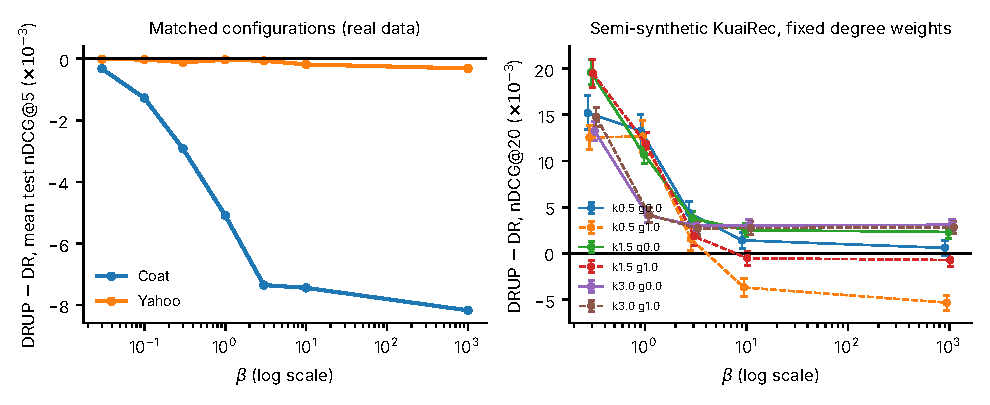
\includegraphics[width=\linewidth]{figs/fig_walk}
\caption{Left: matched-configuration DRUP minus DR adjacency on Coat and Yahoo! R3 against $\beta$ (log scale),
from Table~\ref{tab:walk}. Right: semi-synthetic DRUP minus DR nDCG@20 on KuaiRec for the six cells of the
design, with 95\% CI half-widths; dashed lines are cells with $\gamma=1.0$. Zero lines are shown in both panels.}
\label{fig:walk}
\end{figure}

% Table 7: walk correction. Panel A: results/v3/matched_config_real.txt (values as printed, x1000; shares
% and split counts as printed). Panel B: results/v4/ensemble_summary.txt (Coat lines 3-22; KuaiRec 25-45).
\begin{table}[t]
\centering
\caption{Walk correction and DRUP. Panel A: matched configurations, DRUP minus DR adjacency at the same
configuration, for each value of $\beta$ in the grid, on the real data. Mean differences are $\times10^{-3}$ nDCG@5; ``share $<0$'' is the fraction of the matched
configurations with a negative mean test difference (1{,}440 on Coat, 512 on Yahoo! R3); ``splits $<0$''
counts the splits in which the mean over configurations is negative. Panel B: validated score
ensemble $s=(1-w)\,z(A)+w\,z(\mathrm{DRUP})$, with $z$ standardisation over unlogged items and $w$ chosen per
split on validation data; A is the final method. Holm family of 11 tests within each dataset.}
\label{tab:walk}
\footnotesize
\setlength{\tabcolsep}{2.5pt}
\begin{tabular}{@{}p{4.4cm}rrrrrr@{}}
\toprule
& \multicolumn{3}{c}{Coat} & \multicolumn{3}{c}{Yahoo! R3} \\
\cmidrule(lr){2-4}\cmidrule(lr){5-7}
$\beta$ & Diff & Share & Splits & Diff & Share & Splits \\
\midrule
\multicolumn{7}{@{}l}{\emph{Panel A: matched configurations (DRUP minus DR)}} \\
0.03 & $-0.33$ & 0.49 & 7/10 & $-0.02$ & 0.41 & 5/5 \\
0.1 & $-1.28$ & 0.52 & 9/10 & $-0.03$ & 0.50 & 4/5 \\
0.3 & $-2.92$ & 0.54 & 10/10 & $-0.12$ & 0.56 & 5/5 \\
1.0 & $-5.09$ & 0.74 & 10/10 & $-0.04$ & 0.47 & 3/5 \\
3.0 & $-7.35$ & 0.74 & 10/10 & $-0.07$ & 0.28 & 4/5 \\
10.0 & $-7.44$ & 0.80 & 10/10 & $-0.19$ & 0.41 & 5/5 \\
1000 & $-8.17$ & 0.90 & 10/10 & $-0.32$ & 0.38 & 5/5 \\
\midrule
\multicolumn{7}{@{}l}{\emph{Panel B: validated ensemble with DRUP}} \\
\cmidrule(lr){2-4}\cmidrule(lr){5-7}
& \multicolumn{3}{c}{Coat} & \multicolumn{3}{c}{KuaiRec} \\
\multicolumn{7}{@{}l}{\quad \textit{Test nDCG (mean $\pm$ sd)}} \\
\quad Ensemble $s$ & \multicolumn{3}{c}{0.6031 $\pm$ 0.0164 (Coat)} & \multicolumn{3}{c}{0.6376 $\pm$ 0.0022 (KuaiRec)} \\
\quad A (final), $w=0$ & \multicolumn{3}{c}{0.6015 $\pm$ 0.0162} & \multicolumn{3}{c}{0.6285 $\pm$ 0.0022} \\
\quad DRUP ($w=1$) & \multicolumn{3}{c}{0.5467 $\pm$ 0.0235} & \multicolumn{3}{c}{0.6378 $\pm$ 0.0019} \\
\quad Fixed blend, $w=0.5$ & \multicolumn{3}{c}{0.5889 $\pm$ 0.0134} & \multicolumn{3}{c}{0.6361 $\pm$ 0.0023} \\
\quad Chosen $w$ per split & \multicolumn{3}{c}{0.0 (9 splits), 0.3 (1)} & \multicolumn{3}{c}{0.8 (1 split), 1.0 (4)} \\
\quad $s$ vs A: diff [CI] / $p_{\text{Holm}}$ & \multicolumn{3}{c}{\shortstack{$+1.79$ [2.39]\\$0.1421$}} & \multicolumn{3}{c}{\shortstack{$+8.76$ [2.01]\\$<0.001$}} \\
\quad $s$ vs DRUP: diff [CI] / $p_{\text{Holm}}$ & \multicolumn{3}{c}{\shortstack{$+59.03$ [24.57]\\$<0.001$}} & \multicolumn{3}{c}{\shortstack{$-0.18$ [0.19]\\$0.0664$}} \\
\quad $s$ vs iALS (Coat) / DR-JL (KuaiRec) & \multicolumn{3}{c}{\shortstack{$+21.81$ [20.25]\\$0.0823$}} & \multicolumn{3}{c}{\shortstack{$+4.20$ [2.19]\\$0.0005$}} \\
\bottomrule
\end{tabular}
\end{table}

